%!TEX root = ../thesis.tex

%%% Thesis Introduction --------------------------------------------------
\chapter{Introduction}

\graphicspath{ {Introduction/IntroductionFigs/PNG/}
  {Introduction/IntroductionFigs/PDF/}
  {Introduction/IntroductionFigs/} }

La modélisation géométrique a permis, dans un premier temps, de représenter
des objets virtuels. Des modèles de représentation de nature différente
peuvent être utilisés, comme les surfaces paramétriques ou les maillages. Pour
notre part, nous nous sommes intéressés aux maillages, qui représentent une
discrétisation de l'espace sous forme de cellules (sommets, arêtes, faces,
volumes). Une méthode de déformation naïve consiste à déplacer des sommets
d'un maillage. Mais d'autres types de déformations, plus élaborés, se sont
instaurés. Ils sont pour la plupart propres à une représentation spécifique
d'un maillage, mais certains, comme la déformation \textit{spatiale}, font
abstraction de ces représentations. Nous nous sommes intéressés à ce type de
déformation.
	
La déformation spatiale consiste à déformer un objet en modifiant son espace
ambiant au travers de la modification d'un outil. Cet outil est un ensemble de
points de contrôle (sommets) et les modifications qu'on peut lui appliquer
sont réalisées au travers de la modification de la position de de ces points
de contrôle. Cet outil a des caractéristiques spécifiques, comme sa dimension
(point, courbe, surface, volume), la zone de l'espace qu'il déforme (locale ou
globale) et sa résolution (nombre de points de contrôle). On note \cite{Bar84}
et \cite{SP86} comme étant les premiers à avoir introduit ce type de
déformation. L'avantage de ce procédé, par rapport aux méthodes existantes, a
été de pouvoir réaliser des déformations indépendamment du modèle utilisé pour
représenter l'objet à déformer.

\newpage

En pratique, la déformation d'un objet se décompose en 3 étapes successives:
\begin{enumerate}

\item Construction de l'outil permettant la déformation

\item Association des points de l'espace (composant l'objet) à l'outil
(\textit{temps d'association})

\item Déformation de l'objet par invariance de l'association (\textit{temps de
déformation})

\end{enumerate} 

Les deux premières étapes sont réalisées une seule fois. La dernière étape est
réalisée à chaque manipulation de l'outil de déformation. \\

Ce travail s'inscrit dans une démarche de création d'un nouvel outil de
déformation. Actuellement, pour déformer un objet, les infographistes
utilisent un seul outil à la fois. Mais les différentes déformations ne
peuvent pas toutes être réalisées à l'aide des mêmes outils. Cette contrainte
les force à recréer un nouvel outil lorsque la déformation qu'ils souhaitent
appliquer n'est plus facilement réalisable avec l'outil qu'ils utilisaient
actuellement. Cette étape est une tâche qui peut s'avérer longue et pénible,
d'autant plus que le temps d'association de l'objet à l'outil peut être assez
important. On souhaiterait donc éviter de devoir reproduire cette opération.
L'idée est alors d'avoir un \textit {multi-outil} composé de plusieurs \textit
{sous-outils} communiquant ensemble et déformant chacun diverses zones de
l'objet. A terme, il serait agréable de pouvoir générer automatiquement un
multi-outil en fonction des caractéristiques d'un objet à déformer, afin de
simplifier au maximum le travail des artistes. Dans la suite de ce travail,
nous appelons \textit{outil multidimensionnel}, un multi-outil composé de
plusieurs sous-outils de dimensions différentes. \\

Considérons que notre objet est un alligator (Figure \ref{INTall}), on
souhaite ouvrir la bouche de l'alligator, élargir son ventre et bouger sa
queue, mais ces déformations sont difficilement réalisables avec un seul et
même outil. Pour y parvenir, une bonne solution est de créer un outil
multidimensionnel composé d'axes pour la bouche, d'une cage pour le ventre et
de points pour la queue. Comment mélanger les effets de ces outils de
façon à ce que la déformation engendrée soit visuellement lisse? \\

\begin{figure}[ht]
  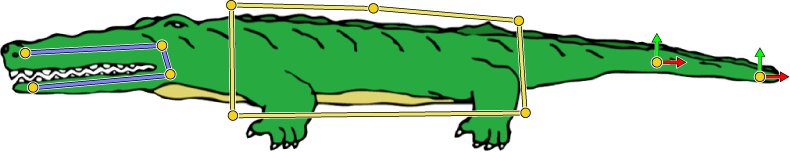
\includegraphics[scale=0.25]{alligator-avant}
  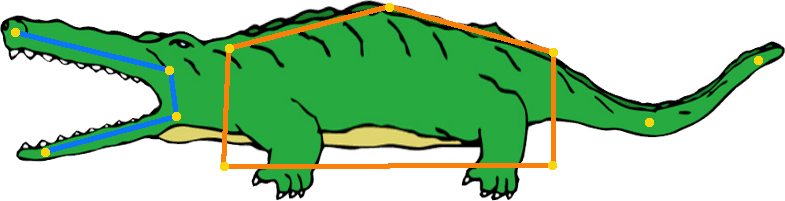
\includegraphics[scale=0.25]{alligator-apres}

  \caption[Explication déformation multi-outil]   {A gauche l'alligator au
temps d'association et à droite après modification de la position de certains
points de contrôle.}

  \label{INTall}
\end{figure}

Afin de guider nos choix quant à la sélection des outils à combiner au travers
d'un multi-outil, nous avons réalisé un état de l'art des outils existants en
se basant en partie sur le travail de \cite{GB08}. Cette partie doit permettre
de faire ressortir un outil pour chacune des dimensions (en fonction de leurs
caractéristiques). Des travaux ont déjà été réalisés sur la partie création
d'un multi-outil par \cite{JBPS11} et \cite{GPCP13}. Les premiers ont mis en
place un outil multidimensionnel se basant sur une méthode d'optimisation
globale, tandis que les autres se sont concentrés sur le mélange d'outils de
déformation de dimension 2. 

Notre travail se situe dans le prolongement de \cite{GPCP13}. L'objectif de ce
stage est de fournir une méthode originale de mélange de différents outils
associés à un même objet. Les points clés sont la minimisation des temps de
calcul (tant au niveau du temps d'association que du temps de déformation)
ainsi que l'élaboration de formules mathématiques simples et claires. Ces
critères ont guidé nos choix lors des différentes étapes de ce travail.
